%\index{\footnote{}}
% Main Content
\chapter{Introduction}

Local governance is fundamental to the upkeep of public infrastructure and the overall well-being of the community. To address public problems such as damaged roads, issues in waste management, street light failures, effective communication between citizens and local authorities is critical. Recently, the integration of e-governance systems and crowdsourcing has improve the citizen participation and streamline the reporting and resolution of public issues. 

However, most of the current systems rely on centralized architectures. This poses a challenge in dealing with data integrity, transparency, and user privacy. Citizens are reluctant to provide complaints about sensitive topics or criticism due to potential retaliation or the possibility of their personal info being abused. At the same time, the local government is faced with the challenge of verifying the authenticity of anonymous complaints raised by citizens.

Some of the key features of Blockchain technology are immutability, transparency, and decentralization. Those features can be used to address several limitations of conventional reporting systems. It is possible to design reporting platforms that protect user anonymity while ensuring the integrity and accountability of reported information by combining blockchain-based architectures and privacy-preserving mechanisms. This project examines the application of blockchain technology in developing a secure, community-driven reporting framework tailored to local governance contexts.


\section{Background}

In the context of local governance, crowdsourced reporting systems and e-governance platforms are widely adopted. By using those systems, citizens can report issues, provide feedback and participate in decision making. It improves the inclusiveness and the accountability of every citizen. In developing countries like Sri Lanka, these systems have the potential to significantly improve the governance efficiency. Timely identification and the resolution of public conccerns are the key to governance efficiency. 

However, despite their advantages, the conventional e-governance and reporting systems are still highly centralized, making them prone to various threats such as data tampering, illegal access, and single points of failure. In addition, the ability to track behavior down to individual users could serve as a discouraging factor, particularly in reporting delicate matters, in a system that lacks anonymity. Blockchain-based systems have appeared as a feasible solution for managing shared data in a tamper-proof and transparent manner. The ability of permissioned blockchains to enable controlled participation while maintaining accountability through trusted validators makes them a desirable choice for governance applications. By using smart contracts, reporting workflows and opinion polling can be automated rather than relying on centralized intermediaries. 

While blockchain technology offers data integrity and transparency, it still poses challenges related to user privacy, content moderation, and trustworthiness among anonymous participants.  These challenges remain open research and implementation problems. Combining  blockchain with privacy-preserving identity mechanisms and \ac{AI}-assisted moderation can help address these limitations and supports the need for a comprehensive framework for secure and reliable community-assisted reporting.

\section{Problem Statement}

The existing frameworks of e-governance and crowdsourced reporting systems for local governance do not provide an integrated mechanism that can guarantee data integrity, user anonymity, and trustworthiness of citizen submitted reports. Centralized architectures are prone to unauthorized access, data tampering, and loss of transparency. At the same time, identity dependent systems discourage citizen engagement due to privacy concerns and fear of retaliation.

Although blockchain has been applied to the context of local government context, many blockchain-based reporting systems still fail to balance anonymity with mechanisms for assessing the reliability and quality of submitted reports. Furthermore, the lack of content moderation and trust evaluation increases the risk of misinformation, and malicious or low quality submissions. 

Therefore, there is a clear need for a privacy-preserving, blockchain-based reporting framework that enables anonymous citizen participation while ensuring data immutability, transparent workflows, and reliable evaluation of reported information. This project aims to address this gap by designing and prototyping a permissioned blockchain-based community-assisted reporting system that incorporates smart contracts, off-chain data storage, and \ac{AI}-assisted content moderation mechanism suitable for local governance environments.



\section{Objectives and Scope}
\subsection{Aim}

The aim of this project is to design and prototype a blockchain-based, privacy-preserving, community-assisted reporting system for local governance that empowers citizens to report public issues and provide their opinions in a transparent, accountable, and secure manner.

\subsection{Objectives}

\begin{enumerate}
\item Design and implement a permissioned reporting blockchain using a \ac{PoA} consensus mechanism to ensure the integrity and immutability of citizen-submitted reports.

% \item Design and deploy smart contracts to automate public issue reporting workflows, including ticket creation, community voting, issue resolution, closure, and public opinion polling.

\item Design and deploy smart contracts to automate public issue reporting workflows, including ticket creation, issue resolution and closure, community voting as feedback on resolved issues, and separate opinion polling mechanisms for public consultation.

\item Develop user-friendly interfaces that enable citizens and authorized government officials to interact with the blockchain for reporting issues and tracking their resolution status.

\item Design and integrate an AI-based content moderation system to detect and filter inappropriate textual and visual content in user-submitted reports.

% \item Analyze user participation behavior and implement an \ac{AI}-assisted trustworthiness evaluation mechanism to improve the reliability of community feedback while preserving user anonymity.

\end{enumerate}


\subsection{Scope}

\begin{enumerate}
   \item A prototype of the proposed blockchain will be implemented with a minimum of three full nodes. The \ac{PoA} consensus mechanism will be used to enable efficient and controlled transaction validation within a permissioned network, while excluding deployment of public, permissionless blockchains or globally distributed ledger infrastructures. 
   
   \item User authentication and identity decoupling are managed through a simulated identity service, and the design and implementation of a fully decentralized Self-Sovereign Identity (SSI) blockchain are explicitly excluded from the scope of this project.
   
   % \item The functional scope of the blockchain layer is strictly limited to managing the lifecycle of reporting tickets  and facilitating public opinion polls, while other e-Governance services such as taxation, civil registration, or licensing systems are not considered. 

   % \item The blockchain is restricted to storing transaction metadata and cryptographic hashes, and the storage of high-capacity data such as images, videos, or detailed \ac{GPS} logs directly on-chain is excluded, with such data instead handled through off-chain storage mechanisms such as \ac{IPFS}.
   
   \item The integration of \ac{AI} within the system is limited to content moderation using existing machine learning models, libraries, or external Application Programming Interfaces (\ac{API}s), and the development of custom, from-scratch deep learning architectures is not within the scope of this work.
   
   % \item The trust evaluation mechanism assesses user reliability solely based on historical reporting behavior and peer-validation voting outcomes, while the incorporation of external data sources such as social media activity, biometric information, or financial credit records is excluded.     % is this needed?
   
   \item Transaction validation authority within the blockchain network is restricted to pre-approved institutional stakeholders, including local government entities and recognized non-governmental organizations, and does not permit anonymous public participation or Proof-of-Work (\ac{PoW}) based mining.
   

   \item The project emphasizes functional validation, system evaluation, and performance analysis within a controlled experimental environment, and does not address real-world legal compliance, regulatory adoption, legislative reform, or large-scale integration with existing national government information systems.

   \item The user interface development is limited to a responsive, web-based \ac{DApp} accessible via standard mobile and desktop web browsers, and explicitly excludes the development of native mobile applications (iOS or Android) or cross-platform native frameworks.

\end{enumerate}


\section{Literature Review}

\subsection{Digital Citizen Reporting and e-Governance Systems}

Electronic governance (e-governance) is using the information and communication technologies to provide government services. This includes the support of government to citizens (G2C), government to business (G2B) , government to agencies (G2A) etc. By utilizing the e-governance platforms, everyone can gain access to whole range of public services. Additionally citizens can submit complaints and participate in governance decision making process. \cite{9587836}.

Digital citizen reporting system is one of the many use case of e-governance. "FixMyStreet" is a a such existing platform. It enable citizens to report issues for different issue categories. Sanitation, Traffic and Public Safety are some examples. Previous studies shows that these kind of systems improve governance administrative efficiency, civic participation and also they increase the transparency.\cite{oliveira2020smartcities}.

Even though there are many benefits of digital citizen reporting in local governance as described earlier, most of them still use centralized server based architecture. This centralized approach have its own limitations and  disadvantages. Susceptibility to data tempering, lack of transparency are the main problems that impact heavily on public trust. In addition to that, mandatory identity disclosure is discouraging public participation on this kind of reporting systems. Therefore these problems motivate the findings of new decentralized, transparent and immutable architectures that still preserve user privacy with accountability.

\subsection{Blockchain for Local Governance Applications}

Blockchain is a technology that has been popular for its ability to have an immutable, transparent and decentralized ledger for public data. Hence, its a transformative tool for e-governance to address the problems that existing implementations had. The Blockchain allow us to verify the immutability of the records, so its suitable for governance applications where the trust and the accountability is crucial. \cite{hamill2018blockchain}, \cite{goswami2020egovernance}.

Blockchain based land registry system implemented in Cook Country, Illinois is a one real world example of the applicability of blockchain in local governance. They aim to reduce the property fraud by consolidating historical ownership records into a verifiable block in the blockchain. Similar to that Delaware has taken initiative to explore the use of smart contracts that's enable real time asset tracking and automate business fillings. This improves the regulatory compliance and oversights \cite{goswami2020egovernance}.

In addition to administrative efficiency, blockchain has been utilized for citizen centric services, such as secure digital identity management. Estonia has taken a initiative to integrate blockchain across healthcare, taxation and even electronic voting systems. So this can provide a mathematically verifiable audit trail for government data. MyPass project in Austin and the World Food Program's building blocks initiative also use Blockchain technology under the hood to manage encrypted identity and transaction records \cite{hamill2018blockchain}.

Despite the advancements in the blockchain base applications, existing literature highlights the challenges of adoption in governance. Scalability constraints, privacy concerns related to identity data, performance overhead and also the need of the legislative and institutional reforms are  some examples. These factors needs to be addressed by carefully selecting blockchain architectures and consensus mechanisms before implementing systems for frequent citizen interactions.

\subsection{Blockchain-Based Citizen Reporting and Complaint Management Systems}

The traditional centralized platforms have data integrity issues, transparency issues and trust issues when it comes to citizen reporting. Past works also indicates that centralized complaint registries often have single point of failures , delayed responses and public mistrust. Therefore blockchain integrated reporting services can be used to mitigate those issues. 

A blockchain based police complaint management system has proposed by Pratheeba \cite{pratheeba_blockchain_police_complaint} contains a modular architecture. It's include security, blockchain, web interface and a hybrid cloud storage. This system ensure immutability of complaint records by cryptographic hash linking. And also it utilize RSA based encryption to restrict the access only to authorized personnel. In Addition to that, Pratheeba used a Natural Language Processing (NLP) techniques to automatically categorize complaints in the system based on their priorities. 

\begin{figure}[h!]
    \centering
    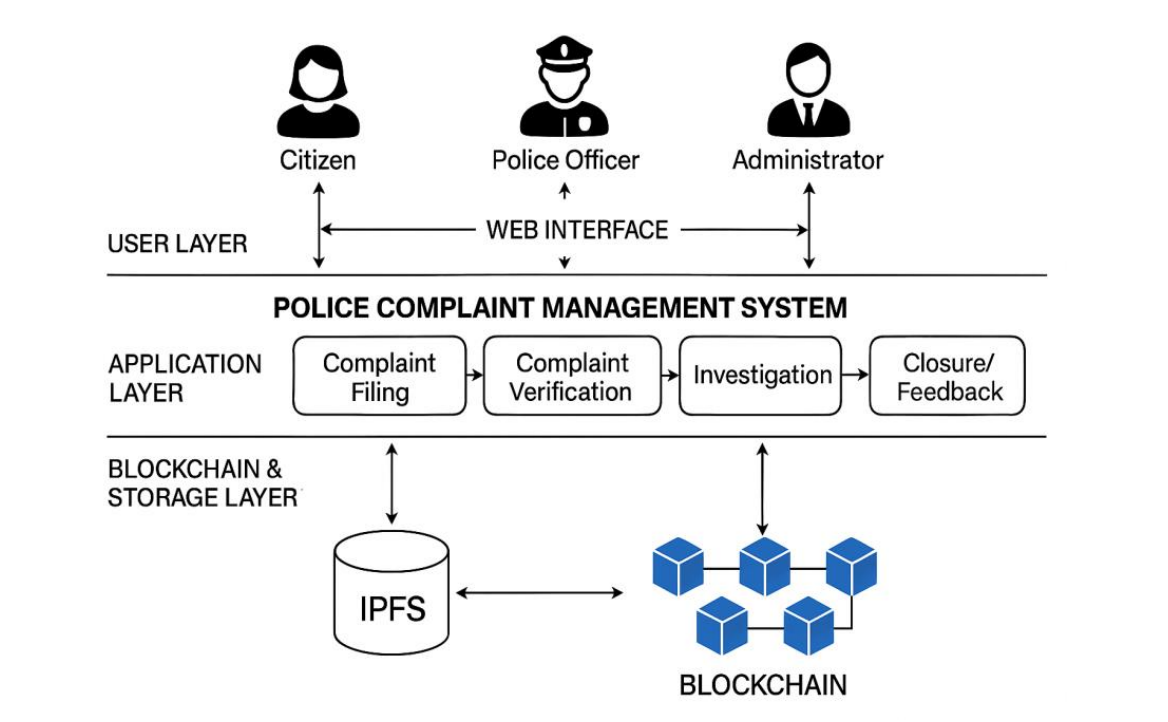
\includegraphics[width=0.95\textwidth]{Images/Chapter 1/system-architecture-police-complaint-system.png} % Replace with your image file
    \caption{System Architecture of the Police Complaint Management System.\cite{manjula2025decentralized}}
    \label{fig:complaint-managment-system-architecture}
\end{figure}


A three tier architecture for decentralized complaint management framework has proposed by Manjula \cite{manjula2025decentralized} is shown in the Figure \ref{fig:complaint-managment-system-architecture}. The three layers are web based presentation layer, a business logic layer and finally a blockchain data layer. This system has a role based access control method to involve multiple stakeholders. Citizens, Law enforcement authorities and judicial bodies are some of them. More importantly this system has a immutable storage for multimedia evidences. Intelligent complaint assignment based on workloads, automatic escalation mechanism are some of the key features of the framework. The experimental evaluations shows that a significant reductions in complaint processing time. The successful detection of data tampering also archived by blockchain verification.

In literature, existing blockchain based complaint management systems shows some improvements in transparency and administrative efficiency. But most of them are domain specific. They primarily target law enforcement or isolated governance functions. In addition to that several platforms still rely on centralized architectures. Only a limited attention is given for implementing a community assisted validation, for privacy preserving reporting mechanisms and efficient handling of multimedia evidences. Therefore these limitations highlight the need for a generalized reporting framework for local governance.

\subsection{Permissioned Blockchains and \ac{PoA} Consensus Mechanisms}

Based on the participation and access control blockchain network can be classified in to two categories.  \cite{und2026commledger}. They are permissionless architecture (public) and permissioned architecture. Bitcoin and Early Ethereum networks are permissionless blockchains. They allowed unrestricted participation and relyed on consensus mechanism like \ac{PoW} or Proof of Stake (\ac{PoS})\cite{mdpi2023survey}. These architectures and consensus mechanisms emphasized decentralization among participants. But they often suffer from the high latency of the network, limited throughput and unpredictable transaction costs due to congestion. These problems make the traditional permissionless PoW or PoS consensus mechanisms unsuitable for governance and crowdsourced applications\cite{arxiv2024performance}.

While permissionless blockchains are unsuitable for governance related applications, permissioned blockchains restrict the network participation to authorized entities. This enables more efficient consensus mechanisms and greater control over governance data \cite{und2026commledger}. This known identities of participants allow permissioned systems to achieve higher performance. And support the regulatory compliances, data privacy and structured governance models as well cite{mdpi2023unleashing}.

Other than \ac{PoW} and \ac{PoS} consensus mechanisms, \ac{PoA} offer significant advantages over permissioned blockchains. \ac{PoW} requires energy intensive computation. \ac{PoS} relies on the economic stake and introduce wealth centralization risks. But on the other hand \ac{PoA} depends on the identity and the reputation of pre approved validators\cite{researchgate2020survey}, \cite{zebpay2026poa}. Therefore this \ac{PoA} consensus mechanism enables high transaction throughput and low latency. And also it mitigate the issues such as the "nothing at stake" problem by off chain legal and reputational accountability \cite{echo2026poa}, \cite{grokipedia2026poa}.

The government systems should have accountability, performance predictability and data confidentiality. The \ac{PoA} is well suited consensus mechanism for that \cite{onekey2026poa}. By using \ac{PoA} we can have the ability to identify and regulate validator entities to align blockchain operations. It's because we have the existing legal frameworks that ensure institutional responsibility. Hence, can avoid malicious behavior \cite{hep2023governance}. In Addition to that PoA avoids the indeterministic transaction fees and support controlled validation environments. This make them viable for handling sensitive governmental data under regulatory constraints\cite{zebpay2026poa},\cite{mdpi2023unleashing}. As a result, \ac{PoA} emerges as a practical consensus mechanism for permissioned blockchain-based reporting systems in local governance contexts.

\subsection{Smart Contracts for Public Issue Management and Opinion Polling}

In governance systems, to improve the transparency, efficiency and citizen participation, smart contracts have been explored as the good mechanism. Smart contracts can automate the governance rules and incentives by immutable code. It can support models like civic intelligence governance (CIG). In CIG, citizen engagement is encouraged through on chain participation and token based incentives\cite{MDPI_2023_CivicIntelligence}. Literature shows that approaches like CIG can improve participation rates and knowledge sharing while reducing relances on centralized intermediaries. In the context of multi organizational governance smart contracts also been used within dual blockchain architectures. This method separates transaction data from contract logic. It balance the transparency and privacy in Government to Government and Business to Business processes\cite{IEEE_2021_SmartCon}.

% Smart contracts also help  business process reengineering in governance processes by directly embedding policy rules into the executable logic. Also the smart contracts help to do the tendering processes and public procurement, automate bid submission, evaluation, and contract execution by making these processes with zero chances for corruption and also increasing the accountability \cite{IEEE_2021_SmartCon}, \cite{GovernanceNow_2023_SmartContractsToolkit}, \cite{AICERTs_2023_FutureOfGovernance}. Also Similar benefits can be seen in blockchain based land registry systems by enabling immutable property records, automated ownership transfers and enforcement of land use policies. So again this reduces the
% fraud and inefficiencies in administratives \cite{ResearchGate_2020_LandRegistry}, \cite{MDPI_2023_NamibianLandRegistration}.

Smart contracts also support business processes in governance by embedding policy rules directly into executable logic. Bid submission, evaluation and contract execution are some of the use cases in the public procurement and tendering processes that smart contract hold its value. It also reduce the oppertunities for corruption and increase the accountability\cite{IEEE_2021_SmartCon}, \cite{GovernanceNow_2023_SmartContractsToolkit}, \cite{AICERTs_2023_FutureOfGovernance}. Similar benefits are observed in the blockchain based land registry systems. Smart contracts have enable immutable property records automated ownership transfers and enforcement of land use policies. This has reduced fraud and administrative inefficiencies\cite{ResearchGate_2020_LandRegistry}, \cite{MDPI_2023_NamibianLandRegistration}.

% If we consider voting and opinion polling, blockchain based systems make sure the security and transparency is protected by ensuring immutability and verifiability of votes while preserving voter anonymity \cite{ResearchGate_2024_ScalableEVoting}, \cite{IEEE_2024_BPVot}. Advanced mechanisms like Quadratic Voting and blockchain enabled participatory budgeting increases the citizen involvement in decision making. They allow more visibility in preference representation and transparent allocation of public resources \cite{ResearchGate_2021_QuadraticVoting}, \cite{UPSpace_2022_ParticipatoryBudgeting}. Eventhough there are many advantages like that, existing studies also highlight some challenges related to scalability, privacy, and system complexity. Particularly when deploying voting and polling solutions for large and diverse populations \cite{ResearchGate_2024_ScalableEVoting}, \cite{JournalOfCybersecurity_2020_BlockchainVoting}.

In the context of voting and opinion polling, smart contracts offer enhanced security, transparency, immutability and verifiability inherited from blockchain\cite{ResearchGate_2024_ScalableEVoting}, \cite{IEEE_2024_BPVot}. There are advance mechanisms such as Quadratic Voting and also blockchain enabled participatory budgeting. Those mechanisms further extend citizen involvement in decision making. It have expressive preference representation and transparent allocation of public resources\cite{ResearchGate_2021_QuadraticVoting}, \cite{UPSpace_2022_ParticipatoryBudgeting}. In addition to these advantages, there exists some challenges related to scalability, privacy and system complexity when deploying voting and polling systems to large and diverse populations\cite{ResearchGate_2024_ScalableEVoting}, \cite{JournalOfCybersecurity_2020_BlockchainVoting}.

\subsection{User Interfaces for Blockchain-Based e-Gover\\nance Applications}

User interfaces play a critical role in determining the accessibility and adoption of blockchain based e-governance systems. In the traditional applications the user literacy is less important but in this conventional blockchain applications the user literacy is highly considered because of the blockchain concepts that are different from the traditional apps and it does make the users hard to understand and adopt. The literature consistently identifies usability and user experience challenges as major barriers to the adoption of decentralized applications for the general public. Particularly where security requirements conflict with established usability principles \cite{mdpi2025usercentric}, \cite{sonule2025uxweb3}. So the design of intuitive, inclusive, and responsive web interfaces is essential for enabling effective interaction between citizens, government officials, and the underlying blockchain infrastructure.

\subsubsection{Usability Challenges in Decentralized Governance Systems}

Decentralized applications are fundamentally different from traditional web systems due to its architectural characteristics. Blockchain based systems have asynchronous transactions, immutable records, and cryptographic identity management. They can create friction for users who are used to centralized platforms. Studies highlight a significant usability gap in Web3 applications because of the concepts like transaction finality, gas fees, and private key ownership which are difficult for non technical users to understand and manage  \cite{mdpi2025usercentric}, \cite{sonule2025uxweb3}.

\subsubsection{Identity Management and Cognitive Load}

One of the most critical usability barriers is wallet based identity management. The reason is user identity is tied to cryptographic key pairs instead of institution managed accounts In decentralized systems. Research shows that the responsibility of safeguarding private keys and the unrecoverble key loss red ce the user participation. Specially in general public where inclusivity is essential \cite{sonule2025uxweb3}, \cite{ramotion2026uiux}, \cite{fintechweekly2025usability}.  

The literature further shows that concepts such as self-sovereign identity and identity management remain poorly understood by most users. Studies report unsafe practices and misunderstanding of recovery mechanisms when users are presented with seed phrases or key-based authentication \cite{oup2022governance}, \cite{fraunhofer2026usability}. These findings motivate the need for interface-level abstractions that preserve blockchain security while reducing cognitive load for citizens and officials.

\subsubsection{Transaction Latency and User Feedback}

Blockchain transactions are inherently asynchronous with confirmation times dependent on network conditions and consensus protocols. This latency can lead to confusion among  the users because of the system status problems and users can determine those as system failures \cite{sonule2025uxweb3}. The literature recommends to use an optimistic user interface pattern, where user actions are acknowledged immediately while blockchain confirmation occurs in the background.  

As advanced design solutions, literature shows progressive status disclosure, distinguishing between off-chain receipt of a report and on-chain verification which allows users to track the lifecycle of an issue without being exposed to unnecessary low level blockchain details \cite{dzone2026blockchainai}, \cite{marian2025transparent}. Mechanisms like that are particularly relevant for issue reporting systems that require transparency and trust.

\subsubsection{Transaction Costs and Abstraction of Blockchain Complexity}

% Another significant usability challenge arises from transaction costs associated with public blockchains. The concept of gas fees and fluctuating costs is unfamiliar in public service contexts, where users expect free access to reporting platforms \cite{mdpi2025usercentric}. The literature strongly supports the use of gas abstraction techniques, such as meta-transactions, where backend relayer services submit transactions on behalf of users while preserving cryptographic intent verification \cite{sonule2025uxweb3}. This approach enables blockchain interaction without exposing citizens to economic or technical complexities.

A significant usability challenge coming from the blockchain is transaction cost that associated with public blockchains. And also the concepts of gas fees and fluctuating gas costs are very unfamiliar in public services context. Most of the time users expect free access to the reporting platforms\cite{mdpi2025usercentric}. The literature strongly suggest that the use of gas fee abstraction techniques. Meta Transactions is one of the example. In Meta, backend relayer services submit transactions on behalf of the user. Its achieved by preserving cryptographic intent verification\cite{sonule2025uxweb3}. Therefore this approach enable citizen to interact with blockchain without technical or economical complexities.


\subsubsection{Comparison with Centralized Reporting Platforms}

% Existing centralized platforms such as FixMyStreet and SeeClickFix provide valuable benchmarks for citizen reporting interfaces. Their success is attributed to intuitive map-based reporting, simple authentication mechanisms, and clear feedback loops that inform users about issue resolution progress \cite{king2012fixmystreet}, \cite{mysociety2026fixmystreet}. SeeClickFix further incorporates gamification mechanisms to encourage participation, although studies caution against over-financializing civic engagement \cite{seeclickfix2011democracy}.  

% In contrast, blockchain-based reporting platforms must reconcile these usability expectations with immutable data storage, decentralized identity, and transparent verification. The literature highlights the need for interface designs that visualize blockchain guarantees such as data integrity and auditability—using familiar metaphors rather than raw cryptographic representations \cite{adeyeye2025blockchain}, \cite {marian2025transparent}, \cite{nikonenko2025blockchain}.  

% Additionally, as multimedia evidence is central to citizen reporting, interfaces must integrate decentralized storage solutions such as InterPlanetary File System (\ac{IPFS}) in a seamless manner, ensuring that large media files are handled off-chain while their integrity is verifiably linked on-chain without exposing technical details to users \cite{mergel2012distributed}, \cite{pazos2024blockchain}.

FixMyStreet and SeeClickFIx are existing centralized platforms. Eventhough they are centralized, they provide a valuable benchmarks for crowdsource citizen reporting interfaces. Inituitive map based reporting, simple authentication mechanisms and clear feedback loops are the key characteristics that attributed to platform success\cite{king2012fixmystreet}, \cite{mysociety2026fixmystreet}.

With addition to that SeeClickFix further uses a gamification mechanism to encourage the users to participate in the system. In contrast, Even though the proposed application uses blockchain for reporting platform, it must retain the usability and the expectations of the users. The literature highlights the need of interface design such that gurantees the data integrity and auditability using familiar ui elements rather than cryptographic representations\cite{adeyeye2025blockchain}, \cite {marian2025transparent}, \cite{nikonenko2025blockchain}.  

% \subsubsection{Trust, Anonymity, and Transparency in Interface Design}

% For privacy-preserving reporting systems, user trust depends not only on protocol guarantees but also on how those guarantees are communicated through the interface. Research on privacy-focused reporting systems emphasizes that users must clearly understand that anonymity is mathematically enforced rather than institutionally promised \cite{lin2023prirpt}. Visual explanations and contextual cues have been shown to improve trust and comprehension more effectively than generic security labels \cite{fraunhofer2026usability}.  

% Similarly, transparency mechanisms such as verification badges, audit timelines, and status indicators help bridge the gap between blockchain-level transparency and human interpretability, enabling users to track issue resolution without interacting directly with block explorers or raw ledger data. \cite{marian2025transparent}, \cite{nikonenko2025blockchain}

\subsubsection{Accessibility and Inclusivity Considerations}

Inclusivity is a fundamental requirement for e-governance systems. According to \cite{bertrand2023connected}, it can be seen that poorly designed blockchain interfaces may digitally divide users. Also it may favor crypto-literate users excluding vulnerable populations. To reduce this issue, literature suggests mobile first design approaches. Furthermore, lightweight client architectures, effiecient bandwidth synchronization can used to support access in resource limited environments.  \cite{shahin2025towards}.  

% The literature warns that poorly designed blockchain interfaces risk exacerbating the digital divide by favoring crypto-literate users and excluding vulnerable populations \cite{bertrand2023connected}. To mitigate this risk, studies advocate mobile-first design approaches, lightweight client architectures, and bandwidth-efficient synchronization to support access in resource-constrained environments \cite{shahin2025towards}.  

% Furthermore, low-code and no-code development platforms are emerging as viable solutions for enabling local governments to deploy and customize reporting interfaces without extensive blockchain expertise, supporting scalability and adaptability across different governance contexts \cite{quixy2025citizen}. These approaches align with the objective of developing user-friendly interfaces that facilitate broad participation and effective interaction with blockchain-based reporting systems.

\subsection{AI-Based Content Moderation in Civic Reporting}

Since blockchain is inheritably immutable its introduce a unique challenge for content moderation in a civic reporting system. In a centralized platforms, administrators can remove or edit inappropriate content. But in a decentralized blockchain based system data cannot be altered once confirmed \cite{tencentcloud2025moderation}. While immutability strengthens transparency and accountability, it also raises the risk of permanently storing harmful, illegal, or misleading content. Therefore the literature focuses the need for pre moderation strategies to prevent unsuitable content from being recorded on chain or to limit its visibility after publication \cite{dzone2026blockchainai}.

\subsection{Need for Automated Content Moderation}

Civic reporting platforms are susceptible to several forms of misuse that can compromise system reliability and public trust. Automated spam submissions, the submission of malicious or legally sensitive content, and deliberate dissemination of false or misleading reports are some of the common issues \cite{wani2024ai}, \cite{gosztonyi2024theory}, \cite{kolluri2025aipowered}. Manual moderation is impractical for above situations. Since the reporting system is large latency, human bias, and operational costs can occur. Furthermore it reintroduces the centralized control structure that blockchain system is aim to minimize. 

Therefore the literature supports AI assisted moderation as a scalable and  efficient approach for filtering content before its permanently recorded. It maintain the acceptable levels of decentralization \cite{mohammadi2025ai}, \cite{goundar2025blockchain}.

\subsection{Architectural Approaches for AI Blockchain Integration}

Due to the computational and storage limitations of blockchain platforms, AI-based moderation cannot be performed directly on chain. Off chain processing combined with on chain verification identified by existing researches as most practical approach\cite{goundar2025blockchain}, \cite{kader2024enhancing}.  

In this approach, reported content is first analyzed by AI models hosted off chain infrastructure or decentralized compute networks. The outcome of this analysis is a validation decision or a trust score. This outcome then submitted to the blockchain as a cryptographic proof or oracle response. Next the smart contracts verify those results before accepting the report. It will ensure that only the content meeting predefined policies are recorded on chain. BlockCITE is a example framework demonstrate how this separation preserves blockchain integrity while avoiding excessive on chain computation \cite{li2025blockcite}.

\subsection{\ac{AI} Oracles and Decentralized Oracle Networks}

Oracles are trusted intermediaries that connect on chain and off chain. In here the \ac{AI} oracles provides the computational results to smart contracts. Instead of simply retrieving external data to the blockchain, \ac{AI} oracle perform content classification and verification tasks. Then it returns the structured results to the blockchain \cite{kava2024aipowered}, \cite{zintusart2025empirical}.  

There can be a risk of oracle bias or failure. To minimize the risk a decentralized oracle networks aggregate outputs from multiple independent \ac{AI} nodes and determine consensus outcomes. This model reduces reliance on a single \ac{AI} system. Therefore it improves te robustness by requiring agreement among multiple validators\cite{zintusart2025empirical}, \cite{codezeros2025aipowered}.

\subsubsection{Techniques for Content Analysis}

\ac{AI}-based moderation techniques vary based on the type of submitted content. \ac{NLP} models are widely used to detect spam, hate speech and misinformation for text based reports. Studies report high accuracy when combining deep learning models with semantic embeddings. It makes them suitable for filtering large volumes of text submissions prior to blockchain recording \cite{wani2024ai}.  

For image based reports computer vision models are used to identify inappropriate contents. However recent advances in generative AI increase the risk of fabricated images. This literature proposes a hybrid verification pipeline that combine cryptographic provenance mechanisms with \ac{AI}-based image analysis. This ensue that the submitted media is both authentic and contextually valid \cite{prasad2024blockchain}.

\subsubsection{Hybrid Human AI Moderation Models}

AI enable the scalable moderation. But it may struggle with contextual interpretation and edge cases. Because of that many studies advocate hybrid moderation models. In those models AI performs initial filtering and prioritization, while human reviewers handle disputed or ambiguous cases \cite{mohammadi2025ai}, \cite{kumar2025hybrid}. 

Decentralized community based moderation further complement this approach. The models using community annotation systems, allow users or designated validators to challenge AI decisions during predefined review periods. In Addition to that dispute resolution handled by transparent governance mechanisms \cite{dzone2026blockchainai}, \cite{kae2025research}. Therefore these strategies reduce the reliance on central authority while maintain the accountability.

\subsubsection{Ethical Considerations and Content Permanence}

Ethical concerns are crucial when implementing systems by integrating AI driven moderation systems. The algorithmic bias and the accountability are the highlights in the literature. Biased training data can lead to unfair rejection of legitimate reports\cite{chase2024ai}. To minimize this risk explainable AI mechanisms are recommended. This enable users to understand the moderation decision and resubmit corrected reports \cite{mounika2024integrated}. 

Finally, the issue of “toxic immutability” remains a critical challenge for blockch\\ain-based systems. To resolve this issue its suggested that to use a off chain storage systems like IPFS. If the content is later identified as illegal or harmful, it can removed from the off chain storage. But can preserve the immutable audit trail by recording it on the blockchain\cite{prasad2024blockchain}. The transparency, legal compliance and ethical responsibility can be balanced by this approach.



\section{Methodology}


\subsection{Research Methodology and Project Approach}

The project uses a design oriented, prototype based research methodology. It develops and evaluates a blockchain based, community assisted, privacy preserving reporting system for local governance. The primary focus is on systematic system design, functional prototyping, and controlled experimental evaluation. It does not focus on large-scale real-world deployment. The methodology follows a structured, step by step system development lifecycle. The workflow begins with requirement analysis and conceptual system design. This is followed by implementation of a permissioned blockchain, smart contracts, off chain services and also AI assisted modules. The system is evaluated and incrementally integrated using functionality metrics and predefined performance and this phased approach ensures traceability between objectives, design decisions, implementation steps, and also evaluation outcomes. Figure~\ref{fig:implementation-methodology} illustrates the overall implementation methodology.

\begin{figure}[h!]
    \centering
    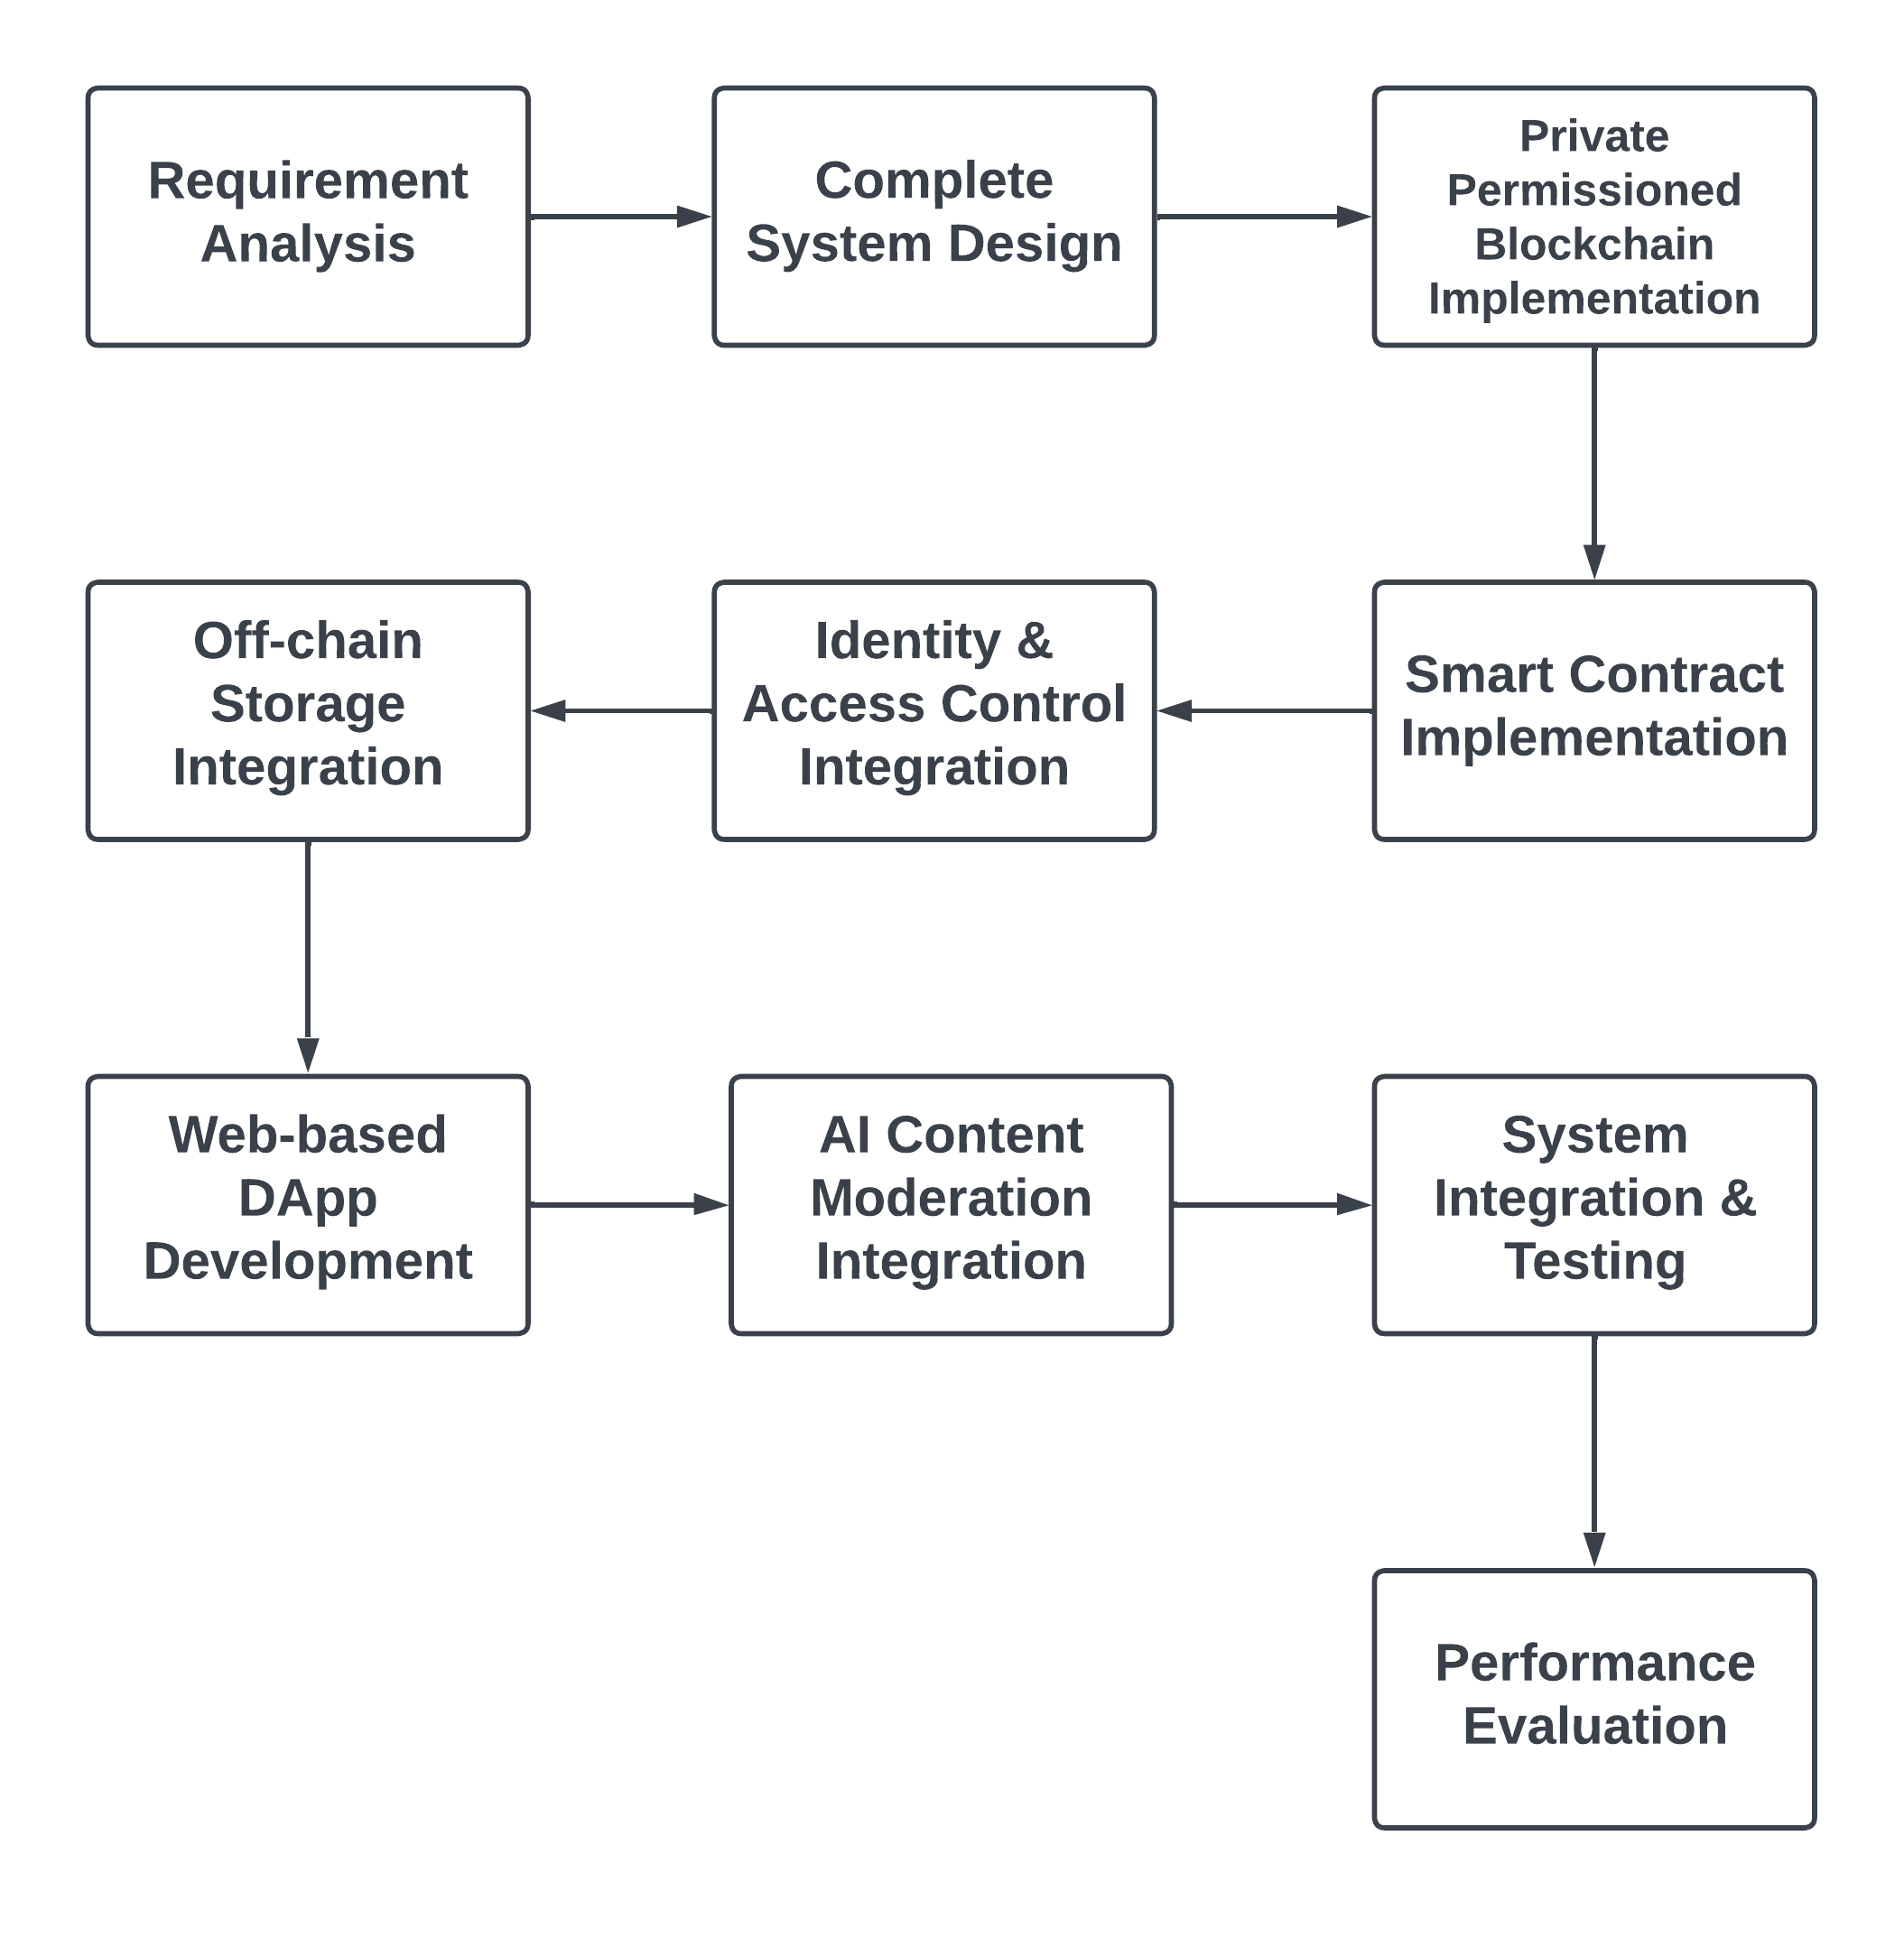
\includegraphics[width=0.95\textwidth]{Images/Chapter 1/implementation-methodology.png}
    \caption{Step-by-Step Implementation Methodology for the Proposed System}
    \label{fig:implementation-methodology}
\end{figure}

\subsection{Requirement Analysis}

Requirement analysis phase identifies functional and non-functional requirements based on project objectives and literature review insights. Citizen issue reporting, community voting, opinion polling, issue tracking, and authority side resolution updates are Functional requirements. Transparency, data integrity, privacy preservation, scalability, and usability are non functional requirements. 

This phase is designed using literature driven requirement extraction approach. Existing blockchain based governance systems and digital reporting platforms are analyzed to get an idea. Use case scenarios for government officials and citizens are defined to guide subsequent system design decisions.

\subsection{Complete System Design}

A comprehensive system design phase is carried out based on identified requirements. The design defines overall architecture, data flows and access control techniques. The system uses a layered architecture. It separates concerns between user interaction, identity management, logics in application, blockchain enforcement, off chain storage, AI services. The architectural design gives modularity for independent development and testing of components. The system design is developed using high level architectural diagrams and workflow. Figure~\ref{fig:architectural-diagram.png} illustrates the high level architecture of the system.

\begin{figure}[h!]
    \centering
    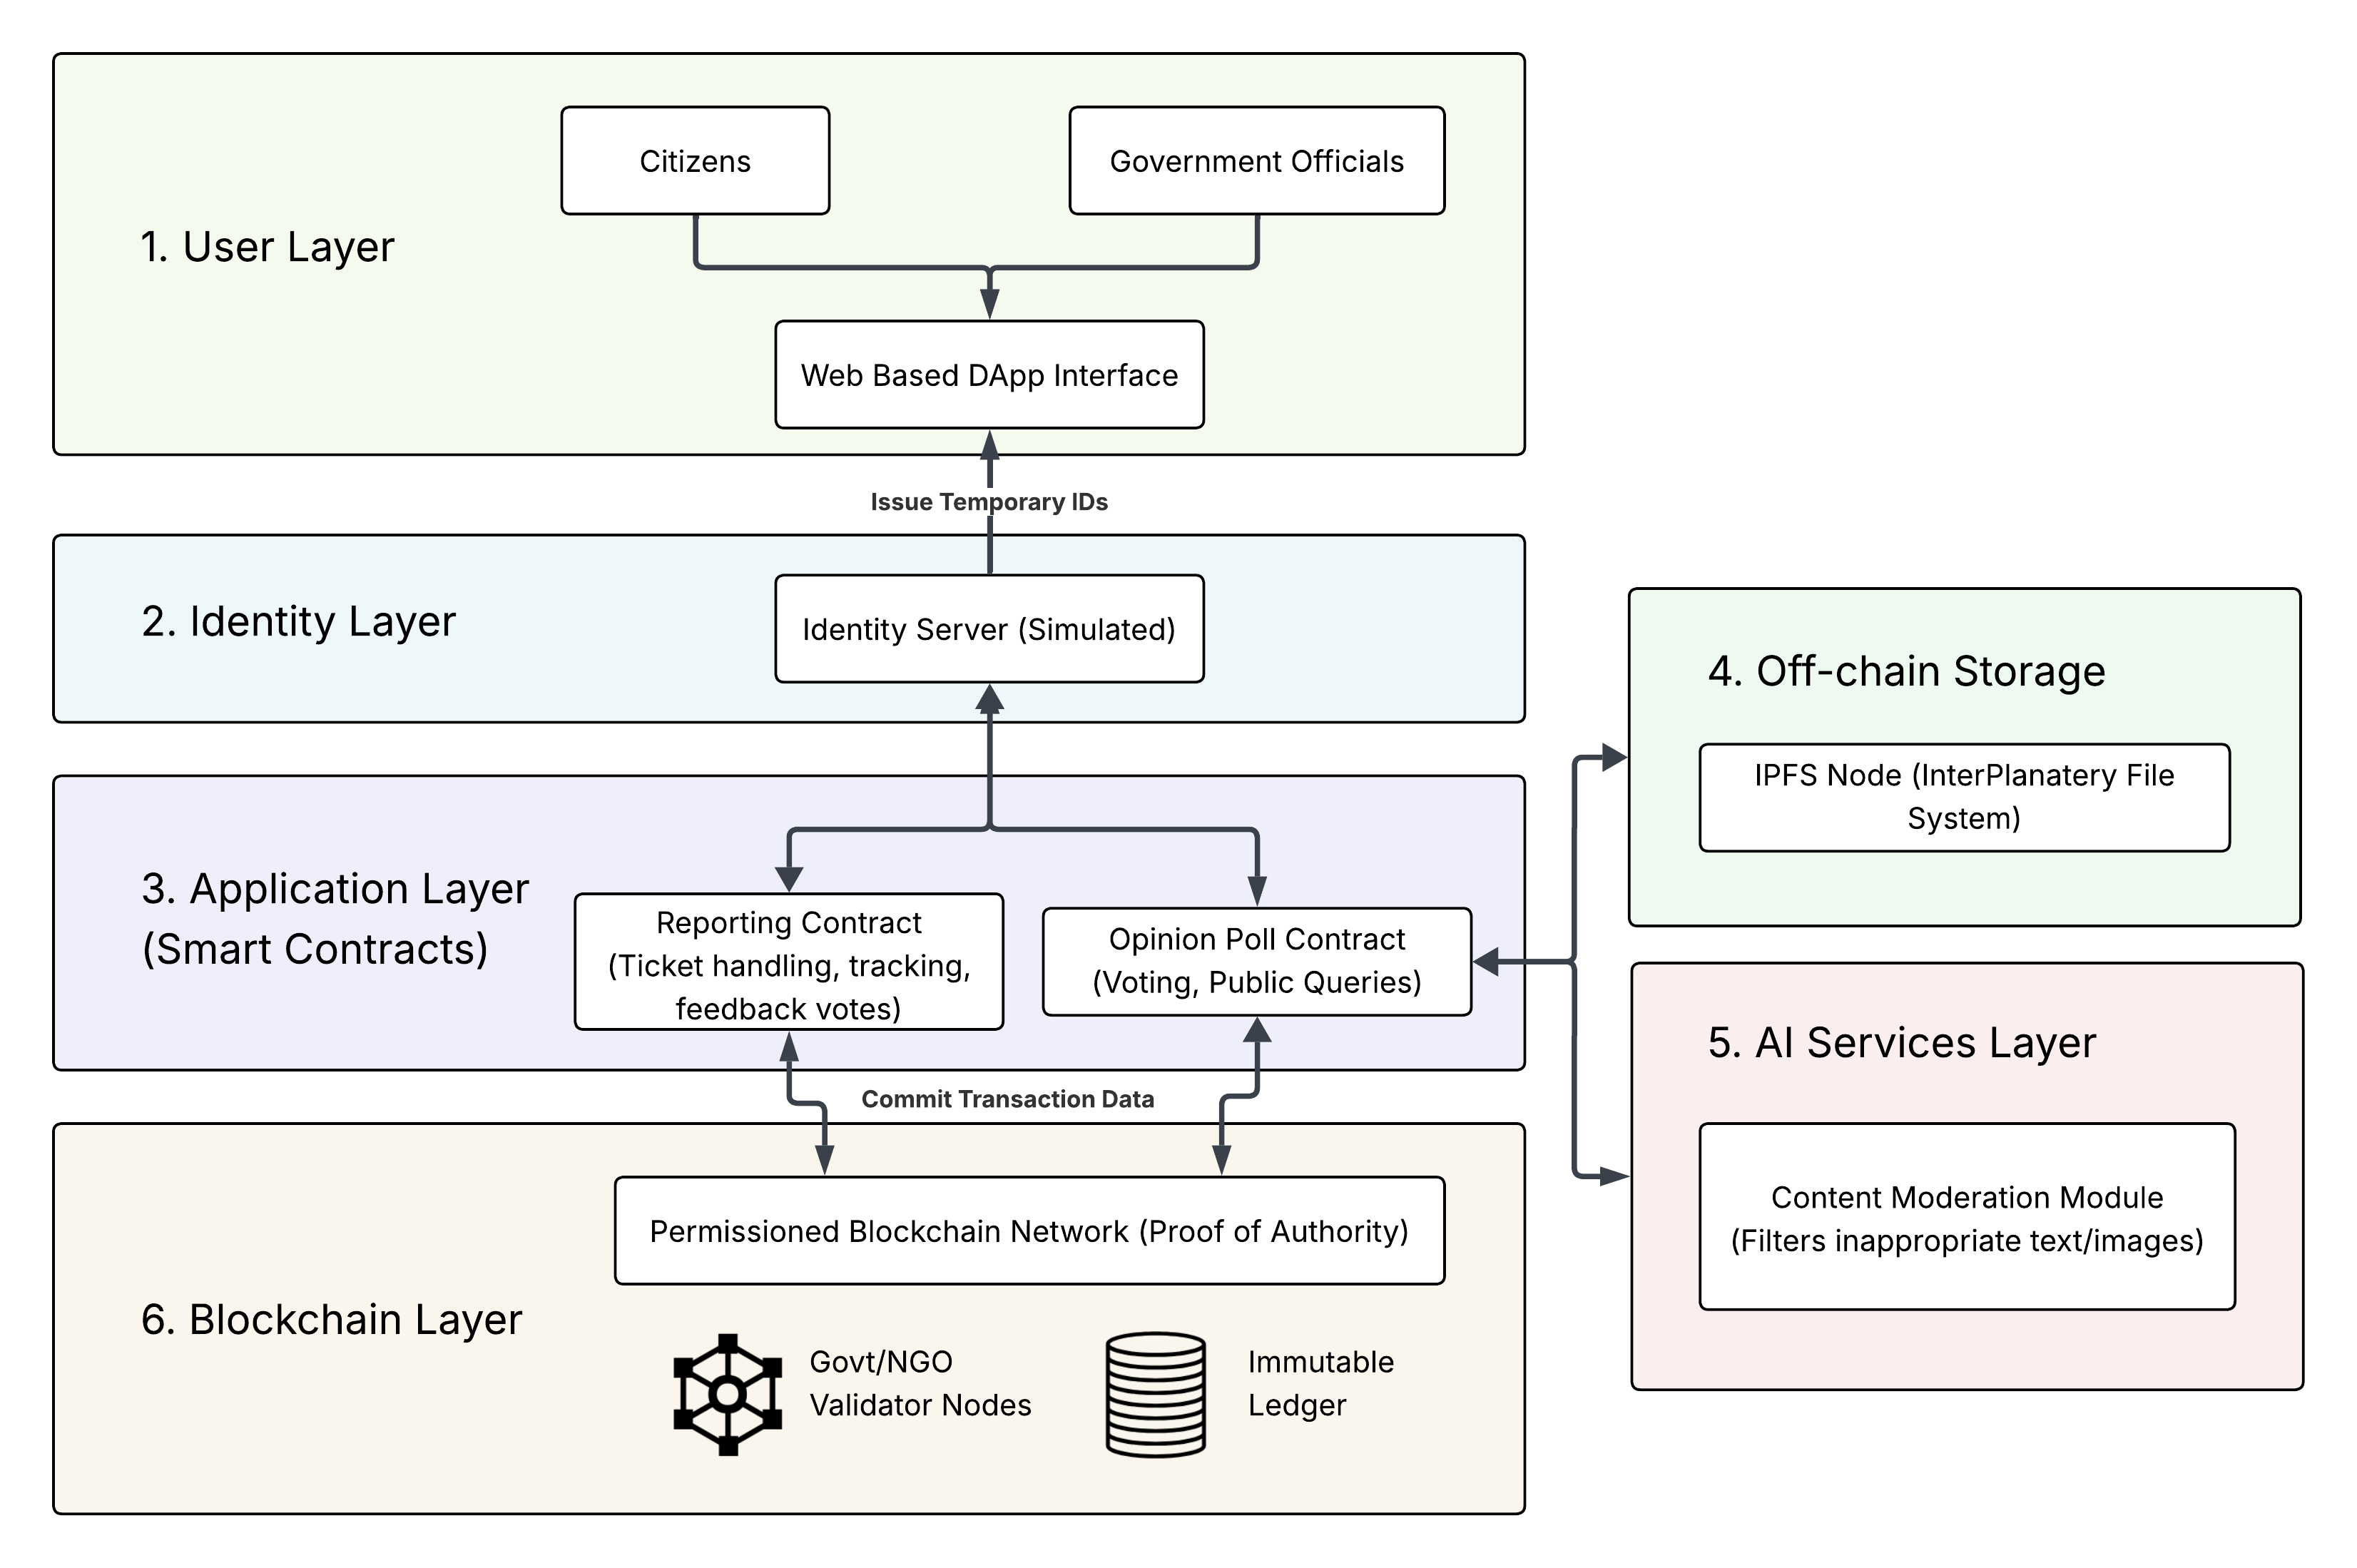
\includegraphics[width=0.95\textwidth]{Images/Chapter 1/architectural-diagram.png}
    \caption{High-Level Architectural Diagram of the Proposed System}
    \label{fig:architectural-diagram.png}
\end{figure}

\subsubsection{Private Permissioned Blockchain Implementation}

A private permissioned blockchain network is implemented to ensure controlled participation, data integrity and also immutability of submitted records. The blockchain operates under a \ac{PoA} consensus mechanism. Validator nodes are assumed to be operated by trusted government or any other organizations. 

The permissioned setup reduces transaction latency and energy consumption compared to public blockchains. The blockchain records report metadata, state transitions, voting, and hashes of off chain content.

\subsubsection{Smart Contract Implementation}

Report submission, ticket creation, community voting, issue status updates, resolution confirmation, closure, and public opinion polling are core reporting workflows of this system. Smart contracts are designed and implemented to automate the above mentioned core reporting workflows. 

The Contracts consider about predefined business logic and access control rules to ensure only authorized users can perform specific actions. Smart contracts are developed using Solidity. permissioned blockchain network is used to deploy Contracts. Contract functionality is tested in a local development environment to validate state transitions and data consistency.

\subsubsection{Identity and Access Control Integration}

A simulated identity and access control mechanism is integrated into the system to preserve user anonymity while enabling accountability. The platform is accessed by the users via pseudonym identifiers distributed by the simulated identity server. Role-Based Access Control differentiates between citizens and government authorities. This is the embodiment of principles of Decoupling Identity without building the full concept of SSI Systems. Verification of identity and access is implemented through application logic and Smart Contract validation.

\subsubsection{Off-chain Storage Integration}

Multimedia content related to reports cannot be recorded on-chain due to limitations of blocks in the blockchain. Therefore, IPFS is used to store multimedia content as a decentralized, off-chain storage. When a user submits a report with multimedia content, the media is uploaded to IPFS and the cryptographic hash related to that media is recorded on-chain via smart contracts. This method ensures data integrity and verifiability of the report. Also it minimizes the on-chain storage overhead and improves the system scalability.

% Due to the storage limitations of blockchain systems, multimedia content such as images and videos associated with reports is stored off-chain. The \ac{IPFS} is used as the decentralized storage solution.


% When a user submits multimedia content, the data is uploaded to IPFS, and the resulting cryptographic hash is recorded on the blockchain via smart contracts. This approach ensures data integrity and verifiability while minimizing on-chain storage overhead and improving system scalability.

\subsubsection{Web-based Decentralized Application Development}

A \ac{DApp} is developed to provide user interfaces for citizens and government officials. By using \ac{DApp} users can submit reports, participate in voting, view issue statuses, and interact with the blockchain network. The frontend is implemented using modern web development frameworks such as Vite, NextJS. Web3 libraries are used to handle blockchain interaction. The \ac{DApp} communicates with smart contracts deployed on the permissioned blockchain and integrates with IPFS and AI module which are stored off-chain.

% \section{Trustworthiness Mechanism Integration}

% To improve the reliability of community participation, a trustworthiness evaluation mechanism is integrated into the system. Trust scores are computed based on user behavior, including historical report validity and peer-validation outcomes.

% The trustworthiness evaluation is performed off-chain using lightweight analytical or AI-assisted models, and the resulting scores influence voting weights and report prioritization. This mechanism enhances data quality while preserving user anonymity and preventing reliance on personal identity data.

\subsubsection{AI-Based Content Moderation Integration}

The AI-based content moderation module is used to detect and filter inappropriate textual and visual content in user-submitted reports. The moderation process is executed off-chain prior to blockchain submission. In this component, existing pretrained AI models or external content moderation APIs are used.

\subsubsection{System Integration and Testing}

To implement the proposed blockchain-based community-assisted reporting system successfully, we need a structured testing procedure. Because blockchain-based records are immutable, bugs introduced in later stages are difficult to correct. Therefore, we will use a testing methodology with early validation and progressive integration throughout the development period. 

The project team will conduct all testing activities within a controlled environment. Each subsystem is tested by the team member responsible for its design and implementation. It is followed by joint integration testing to ensure all modules interact correctly. 

\subsubsection{Testing Responsibilities and Approach}

Testing responsibilities are distributed according to system functionality. The project team performs the following testing tasks collectively. 
\begin{enumerate}[i]
    \item Blockchain and smart contract testing. (transaction execution,
    access control, workflow validation)
    \item Web interface testing (user interactions, data submission, status visualization)
    \item AI module testing (appropriate filtering of textual and visual
    content)
    \item Integration testing (data flow across the blockchain, AI services,
    off-chain storage, and user interface layers)
\end{enumerate}

\subsubsection{Data Acquisition and Test Data Generation}

Because the system is evaluated within a controlled experimental environment, testing relies on a combination of synthetic data and publicly available datasets. The different categories of test data used in the project and their purposes are summarized in Table~\ref{tab:data-acquisition}.

\begin{table}[h!]
\centering
\small
\renewcommand{\arraystretch}{1.4}
\caption{Test Data Sources and Usage}
\label{tab:data-acquisition}
\begin{tabular}{|p{4cm}|p{4cm}|p{5cm}|}
\hline
\textbf{Data Type} & \textbf{Data Source} & \textbf{Purpose in Testing} \\ \hline

Synthetic Reporting Data &
Programmatically generated using scripts and mock user profiles &
Simulation of citizen reports, voting actions, issue resolution events, and validation of blockchain workflows and smart contract execution \\ \hline

Textual Content Samples &
Publicly available moderation datasets and manually curated samples &
Evaluation of AI-based text moderation for detecting inappropriate, irrelevant, or malicious textual content \\ \hline

Visual Evidence Samples &
Public urban infrastructure datasets (e.g., potholes, garbage, road damage images) &
Testing image-based content moderation, off-chain storage via IPFS, and hash integrity verification \\ \hline

\end{tabular}
\end{table}


The use of synthetic and publicly available datasets ensures ethical compliance,
repeatability, and controlled experimentation.

\subsubsection{Subsystem-Level Testing}

According to the Table \ref{tab:testing-plan}, all major subsystems are tested independently before full system integration.

\begin{table}[h!]
\centering
\small
\renewcommand{\arraystretch}{1.4}
\caption{Subsystems and Planned Testing Activities}
\label{tab:testing-plan}
\begin{tabular}{|p{5.5cm}|p{7.5cm}|}
\hline
\textbf{Subsystem} & \textbf{Testing Method} \\ \hline

Permissioned Blockchain Network &
Functional testing of transaction validation, block creation, and validator authorization under PoA consensus \\ \hline

Smart Contract Logic &
Unit testing of report creation, feedback voting, status transitions, issue closure, and opinion polling workflows \\ \hline

User Interface Module &
Functional and usability testing of report submission, issue tracking, feedback voting, and polling interactions \\ \hline

AI-Based Content Moderation &
Validation of text and image filtering accuracy using synthetic and public datasets \\ \hline

Off-Chain Storage Module &
Testing of file uploads, hash generation, and integrity verification between IPFS and blockchain \\ \hline

End-to-End System Integration &
Scenario-based testing of complete workflows from report submission to issue closure  \\ \hline

\end{tabular}
\end{table}

\subsubsection{System Integration Testing}

After successful subsystem testing, end-to-end integration testing is performed.
Complete reporting scenarios are simulated, starting from report submission and
content moderation to blockchain recording, community feedback voting, issue
resolution updates, and final closure.

In the integration test, we mainly focus on  consistent data flow, correct state
synchronization, and reliable interaction between all system components.

\subsubsection{Performance Evaluation}

% The performance evaluation assesses the operational feasibility of the proposed
% system within a controlled experimental environment. The objective is not to
% benchmark production-level performance but to demonstrate that the architecture
% can reliably support community-assisted reporting workflows.
The performance evaluation evaluates the operational feasibility of the proposed system within a controlled experimental environment. The objective is to demonstrate that the architecture can reliably support community-assisted reporting workflows. It will not benchmark production-level performance. 

\subsection{Evaluation Environment}

The evaluation environment consists of a private, Ethereum-compatible blockchain network. This network is configured with a \ac{PoA} consensus mechanism. We will test the system using simulated users and synthetic workloads generated by the project team.

\subsubsection{Evaluation Metrics}

The performance and reliability of the proposed system are evaluated using the evaluation metrics stated in the Table~\ref{tab:evaluation-metrics}.

\begin{table}[h!]
\centering
\small
\renewcommand{\arraystretch}{1.4}
\caption{System Evaluation Metrics}
\label{tab:evaluation-metrics}
\begin{tabular}{|p{4cm}|p{10cm}|}
\hline
\textbf{Metric} & \textbf{Description} \\ \hline

Transaction Latency &
Time required for report submissions, voting actions, and status updates to be
confirmed on the blockchain \\ \hline

Transaction Throughput &
Number of transactions processed per unit time during simulated reporting and
community voting activity  \\ \hline

Smart Contract Execution Reliability &
Consistency and correctness of smart contract execution during repeated workflow
operations \\ \hline

AI Moderation Response Time &
Time taken for text-based and image-based content moderation decisions to be
returned and integrated into the workflow  \\ \hline

Off-Chain Storage Performance &
Time required to upload and retrieve multimedia evidence from off-chain storage  \\ \hline

\end{tabular}
\end{table}


\subsubsection{Testing Procedure}

Performance testing is conducted by gradually increasing the number of simulated reports and feedback votes submitted to the system. All transaction logs and execution results are recorded. Those records will then be analyzed to observe latency trends, system stability, and failure conditions.

\subsection{Limitations}

The performance evaluation is limited to prototype deployment using simulated
data in a controlled environment. Real-world network conditions, large-scale user
adoption, and institutional deployment constraints are outside the scope of this
project. 


\section{Time Plan and Resources Required}


\subsection{Project Timeline}

The project is planned to be completed over two academic semesters following
a structured and incremental development approach as shown in Figure \ref{fig:ganttchart}. The timeline allocates
sufficient time for system design, implementation, testing, evaluation to ensure the successful completion of the proposed objectives.


\subsection{Resources Required}

The successful implementation and evaluation of the proposed system require a combination of computational resources, software tools, and development platforms. As the project focuses on prototyping and experimental validation, the required resources are limited to a controlled academic environment. 


\begin{enumerate}[i]
    \item Three university-provided high-compute machines to simulate a permissioned blockchain network.

    \item Personal laptops for application development, testing, and documentation.

    \item Ethereum-compatible permissioned blockchain framework configured with \ac{PoA} consensus.

    \item Smart contract development tools (Solidity, Hardhat/Truffle, Remix).

    \item Modern web application development technologies for building a responsive and user-friendly \ac{DApp} interface.

    \item Python-based machine learning libraries and pre-trained models for
    content moderation.

    \item \ac{IPFS} for off-chain multimedia storage.

    \item Version control and collaboration tools (Git, GitHub).
\end{enumerate}


% \begin{sidewaysfigure}[p]
%     \centering
%     % Resize the chart to fit the page height (which is width in landscape)
%     \resizebox{\textwidth}{!}{%
    
%     \begin{ganttchart}[
%         % --- Chart Settings ---
%         vgrid={*1{draw=gridgray}},
%         hgrid={draw=gridgray},
%         y unit chart=0.7cm,      % Reduced slightly to fit vertical space
%         x unit=0.4cm,            
%         title label font=\color{black},
%         title/.style={draw=gray!50, line width=0.5pt},
%         title height=1,
%         include title in canvas=false,
%         bar/.style={fill=barblue, draw=none},
%         bar height=0.7,
%         group right shift=0,
%         group top shift=0.7,
%         group height=.3,
%         % Label box styling
%         label node/.style={
%             fill=labelgray, 
%             draw=gridgray, 
%             inner sep=3pt, 
%             font=\sffamily\footnotesize
%         }
%         ]{1}{37}

%         % --- HEADERS ---
%         %\gantttitle[title/.style={fill=white, draw=none}]{WEEK}{37} \\
%         \gantttitle{NOV}{3}
%         \gantttitle{DEC}{4}
%         \gantttitle{JAN}{4}
%         \gantttitle{FEB}{4}
%         \gantttitle{MAR}{4}
%         \gantttitle{APR}{4}
%         \gantttitle{MAY}{4}
%         \gantttitle{JUNE}{4}
%         \gantttitle{JULY}{4}
%         \gantttitle{AUG}{2} \\
%         \gantttitlelist[title label font=\color{black}\scriptsize]{1,...,37}{1} \\

%         % --- TASKS ---
%         % Usage: \ganttbar{\ganttlabel{Title}{Owner}}{Start}{End}
%         % --- COLUMN HEADERS FOR TASK LABELS ---

%         \ganttbar{\ganttlabel{Grouping \& Project Selection}}{1}{2} \\
%         \ganttbar{\ganttlabel{Background Study }}{2}{4} \\
%         \ganttbar{\ganttlabel{Literature Study}}{5}{9} \\
%         \ganttbar{\ganttlabel{Project Proposal}}{9}{10} \\
%         \ganttbar{\ganttlabel{Project Proposal Evaluation}}{10}{11} \\
%         \ganttbar{\ganttlabel{Complete System Design}}{11}{14} \\
%         \ganttbar{\ganttlabel{Permissioned Blockchain Implementation}}{14}{19} \\
%         \ganttbar{\ganttlabel{Smart Contract Implementation}}{19}{23} \\
%         \ganttbar{\ganttlabel{Identity \& Access Control Integration}}{17}{20} \\
%         \ganttbar{\ganttlabel{Off-chain Storage Integration}}{22}{25} \\
%         \ganttbar{\ganttlabel{AI Content Moderation Integration}}{13}{17} \\
%         % \ganttbar{\ganttlabel{Trustworthiness Mechanism Integration}}{22}{27} \\
%         \ganttbar{\ganttlabel{Web-based DApp Development}}{16}{31} \\
%         \ganttbar{\ganttlabel{System Integration \& Testing}}{30}{34} \\
%         \ganttbar{\ganttlabel{Performance Evaluation}}{34}{36} \\
%         \ganttbar{\ganttlabel{Final Demonstration}}{36}{37}

%     \end{ganttchart}
%     } % End of resizebox
    
%     \caption{Project Timeline Gantt Chart}
%     \label{fig:ganttchart}
% \end{sidewaysfigure}

\begin{sidewaysfigure}[p]
    \centering
    \resizebox{\textwidth}{!}{%
    
    \begin{ganttchart}[
        vgrid={*1{draw=gridgray}},
        hgrid={draw=gridgray},
        y unit chart=0.7cm,
        x unit=0.4cm,
        title label font=\color{black},
        title/.style={draw=gray!50, line width=0.5pt},
        title height=1,
        include title in canvas=false,
        bar/.style={fill=barblue, draw=none},
        bar height=0.7,
        group right shift=0,
        group top shift=0.7,
        group height=.3,
        label node/.style={
            fill=labelgray,
            draw=gridgray,
            inner sep=3pt,
            font=\sffamily\footnotesize
        }
        ]{1}{37}

        % --- HEADERS ---
        \gantttitle{NOV}{3}
        \gantttitle{DEC}{4}
        \gantttitle{JAN}{4}
        \gantttitle{FEB}{4}
        \gantttitle{MAR}{4}
        \gantttitle{APR}{4}
        \gantttitle{MAY}{4}
        \gantttitle{JUNE}{4}
        \gantttitle{JULY}{4}
        \gantttitle{AUG}{2} \\
        \gantttitlelist[title label font=\color{black}\scriptsize]{1,...,37}{1} \\

        % --- METHODOLOGY-ALIGNED TASKS ---

        \ganttbar{\ganttlabel{Grouping \& Project Selection}}{1}{2} \\
        \ganttbar{\ganttlabel{Background Study}}{2}{4} \\
        \ganttbar{\ganttlabel{Literature Review}}{4}{8} \\
        \ganttbar{\ganttlabel{Requirement Analysis}}{7}{10} \\
        \ganttbar{\ganttlabel{Project Proposal Preparation}}{9}{10} \\
        \ganttbar{\ganttlabel{Proposal Evaluation}}{10}{11} \\

        \ganttbar{\ganttlabel{Complete System Design}}{11}{15} \\

        \ganttbar{\ganttlabel{Permissioned Blockchain Setup}}{15}{20} \\
        \ganttbar{\ganttlabel{Smart Contract Development}}{18}{24} \\
        \ganttbar{\ganttlabel{Identity \& Access Control Integration}}{19}{23} \\
        \ganttbar{\ganttlabel{\ac{IPFS} Integration}}{22}{26} \\
        \ganttbar{\ganttlabel{AI-Based Content Moderation Integration}}{16}{21} \\

        \ganttbar{\ganttlabel{Web-based \ac{DApp} Development}}{18}{30} \\

        \ganttbar{\ganttlabel{Subsystem Testing}}{26}{30} \\
        \ganttbar{\ganttlabel{System Integration \& End-to-End Testing}}{30}{34} \\

        \ganttbar{\ganttlabel{Performance Evaluation}}{34}{36} \\
        \ganttbar{\ganttlabel{Final Demonstration}}{36}{37}

    \end{ganttchart}
    }
    \caption{Project Timeline Gantt Chart}
    \label{fig:ganttchart}
\end{sidewaysfigure}




%%%%%%%%%%%%%%%%%%%%%%%%%%%%%%%%%%%%%%%%%%%%%%%%%%%%%%%%%%%%%%%%%%%%%%%%%%%%%%%%%%%%%%%%%%%%%%%%%%
%%%%%%%%%%% END OF FILE
%%%%%%%%%%%%%%%%%%%%%%%%%%%%%%%%%%%%%%%%%%%%%%%%%%%%%%%%%%%%%%%%%%%%%%%%%%%%%%%%%%%%%%%%%%%%%%%%%%
